\documentclass[1p]{elsarticle_modified}
%\bibliographystyle{elsarticle-num}

%\usepackage[colorlinks]{hyperref}
%\usepackage{abbrmath_seonhwa} %\Abb, \Ascr, \Acal ,\Abf, \Afrak
\usepackage{amsfonts}
\usepackage{amssymb}
\usepackage{amsmath}
\usepackage{amsthm}
\usepackage{scalefnt}
\usepackage{amsbsy}
\usepackage{kotex}
\usepackage{caption}
\usepackage{subfig}
\usepackage{color}
\usepackage{graphicx}
\usepackage{xcolor} %% white, black, red, green, blue, cyan, magenta, yellow
\usepackage{float}
\usepackage{setspace}
\usepackage{hyperref}

\usepackage{tikz}
\usetikzlibrary{arrows}

\usepackage{multirow}
\usepackage{array} % fixed length table
\usepackage{hhline}

%%%%%%%%%%%%%%%%%%%%%
\makeatletter
\renewcommand*\env@matrix[1][\arraystretch]{%
	\edef\arraystretch{#1}%
	\hskip -\arraycolsep
	\let\@ifnextchar\new@ifnextchar
	\array{*\c@MaxMatrixCols c}}
\makeatother %https://tex.stackexchange.com/questions/14071/how-can-i-increase-the-line-spacing-in-a-matrix
%%%%%%%%%%%%%%%

\usepackage[normalem]{ulem}

\newcommand{\msout}[1]{\ifmmode\text{\sout{\ensuremath{#1}}}\else\sout{#1}\fi}
%SOURCE: \msout is \stkout macro in https://tex.stackexchange.com/questions/20609/strikeout-in-math-mode

\newcommand{\cancel}[1]{
	\ifmmode
	{\color{red}\msout{#1}}
	\else
	{\color{red}\sout{#1}}
	\fi
}

\newcommand{\add}[1]{
	{\color{blue}\uwave{#1}}
}

\newcommand{\replace}[2]{
	\ifmmode
	{\color{red}\msout{#1}}{\color{blue}\uwave{#2}}
	\else
	{\color{red}\sout{#1}}{\color{blue}\uwave{#2}}
	\fi
}

\newcommand{\Sol}{\mathcal{S}} %segment
\newcommand{\D}{D} %diagram
\newcommand{\A}{\mathcal{A}} %arc


%%%%%%%%%%%%%%%%%%%%%%%%%%%%%5 test

\def\sl{\operatorname{\textup{SL}}(2,\Cbb)}
\def\psl{\operatorname{\textup{PSL}}(2,\Cbb)}
\def\quan{\mkern 1mu \triangleright \mkern 1mu}

\theoremstyle{definition}
\newtheorem{thm}{Theorem}[section]
\newtheorem{prop}[thm]{Proposition}
\newtheorem{lem}[thm]{Lemma}
\newtheorem{ques}[thm]{Question}
\newtheorem{cor}[thm]{Corollary}
\newtheorem{defn}[thm]{Definition}
\newtheorem{exam}[thm]{Example}
\newtheorem{rmk}[thm]{Remark}
\newtheorem{alg}[thm]{Algorithm}

\newcommand{\I}{\sqrt{-1}}
\begin{document}

%\begin{frontmatter}
%
%\title{Boundary parabolic representations of knots up to 8 crossings}
%
%%% Group authors per affiliation:
%\author{Yunhi Cho} 
%\address{Department of Mathematics, University of Seoul, Seoul, Korea}
%\ead{yhcho@uos.ac.kr}
%
%
%\author{Seonhwa Kim} %\fnref{s_kim}}
%\address{Center for Geometry and Physics, Institute for Basic Science, Pohang, 37673, Korea}
%\ead{ryeona17@ibs.re.kr}
%
%\author{Hyuk Kim}
%\address{Department of Mathematical Sciences, Seoul National University, Seoul 08826, Korea}
%\ead{hyukkim@snu.ac.kr}
%
%\author{Seokbeom Yoon}
%\address{Department of Mathematical Sciences, Seoul National University, Seoul, 08826,  Korea}
%\ead{sbyoon15@snu.ac.kr}
%
%\begin{abstract}
%We find all boundary parabolic representation of knots up to 8 crossings.
%
%\end{abstract}
%\begin{keyword}
%    \MSC[2010] 57M25 
%\end{keyword}
%
%\end{frontmatter}

%\linenumbers
%\tableofcontents
%
\newcommand\colored[1]{\textcolor{white}{\rule[-0.35ex]{0.8em}{1.4ex}}\kern-0.8em\color{red} #1}%
%\newcommand\colored[1]{\textcolor{white}{ #1}\kern-2.17ex	\textcolor{white}{ #1}\kern-1.81ex	\textcolor{white}{ #1}\kern-2.15ex\color{red}#1	}

{\Large $\underline{12a_{0691}~(K12a_{0691})}$}

\setlength{\tabcolsep}{10pt}
\renewcommand{\arraystretch}{1.6}
\vspace{1cm}\begin{tabular}{m{100pt}>{\centering\arraybackslash}m{274pt}}
\multirow{5}{120pt}{
	\centering
	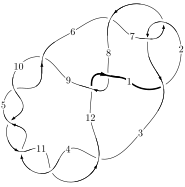
\includegraphics[width=112pt]{../../../GIT/diagram.site/Diagrams/png/1492_12a_0691.png}\\
\ \ \ A knot diagram\footnotemark}&
\allowdisplaybreaks
\textbf{Linearized knot diagam} \\
\cline{2-2}
 &
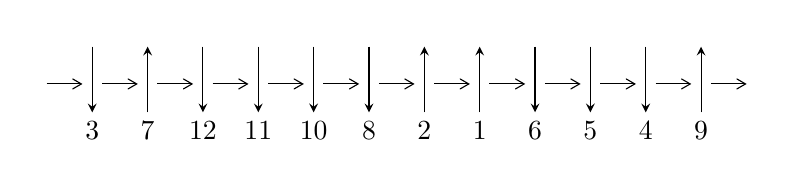
\begin{tikzpicture}[x=20pt, y=17pt]
	% nodes
	\node (C0) at (0, 0) {};
	\node (C1) at (1, 0) {};
	\node (C1U) at (1, +1) {};
	\node (C1D) at (1, -1) {3};

	\node (C2) at (2, 0) {};
	\node (C2U) at (2, +1) {};
	\node (C2D) at (2, -1) {7};

	\node (C3) at (3, 0) {};
	\node (C3U) at (3, +1) {};
	\node (C3D) at (3, -1) {12};

	\node (C4) at (4, 0) {};
	\node (C4U) at (4, +1) {};
	\node (C4D) at (4, -1) {11};

	\node (C5) at (5, 0) {};
	\node (C5U) at (5, +1) {};
	\node (C5D) at (5, -1) {10};

	\node (C6) at (6, 0) {};
	\node (C6U) at (6, +1) {};
	\node (C6D) at (6, -1) {8};

	\node (C7) at (7, 0) {};
	\node (C7U) at (7, +1) {};
	\node (C7D) at (7, -1) {2};

	\node (C8) at (8, 0) {};
	\node (C8U) at (8, +1) {};
	\node (C8D) at (8, -1) {1};

	\node (C9) at (9, 0) {};
	\node (C9U) at (9, +1) {};
	\node (C9D) at (9, -1) {6};

	\node (C10) at (10, 0) {};
	\node (C10U) at (10, +1) {};
	\node (C10D) at (10, -1) {5};

	\node (C11) at (11, 0) {};
	\node (C11U) at (11, +1) {};
	\node (C11D) at (11, -1) {4};

	\node (C12) at (12, 0) {};
	\node (C12U) at (12, +1) {};
	\node (C12D) at (12, -1) {9};
	\node (C13) at (13, 0) {};

	% arrows
	\draw[->,>={angle 60}]
	(C0) edge (C1) (C1) edge (C2) (C2) edge (C3) (C3) edge (C4) (C4) edge (C5) (C5) edge (C6) (C6) edge (C7) (C7) edge (C8) (C8) edge (C9) (C9) edge (C10) (C10) edge (C11) (C11) edge (C12) (C12) edge (C13) ;	\draw[->,>=stealth]
	(C1U) edge (C1D) (C2D) edge (C2U) (C3U) edge (C3D) (C4U) edge (C4D) (C5U) edge (C5D) (C6U) edge (C6D) (C7D) edge (C7U) (C8D) edge (C8U) (C9U) edge (C9D) (C10U) edge (C10D) (C11U) edge (C11D) (C12D) edge (C12U) ;
	\end{tikzpicture} \\
\hhline{~~} \\& 
\textbf{Solving Sequence} \\ \cline{2-2} 
 &
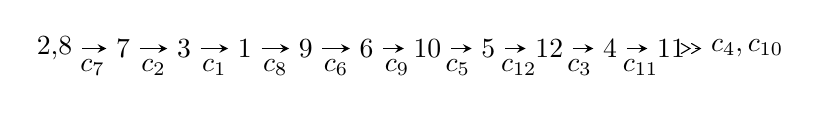
\begin{tikzpicture}[x=22pt, y=7pt]
	% node
	\node (A0) at (-1/8, 0) {2,8};
	\node (A1) at (1, 0) {7};
	\node (A2) at (2, 0) {3};
	\node (A3) at (3, 0) {1};
	\node (A4) at (4, 0) {9};
	\node (A5) at (5, 0) {6};
	\node (A6) at (6, 0) {10};
	\node (A7) at (7, 0) {5};
	\node (A8) at (8, 0) {12};
	\node (A9) at (9, 0) {4};
	\node (A10) at (10, 0) {11};
	\node (C1) at (1/2, -1) {$c_{7}$};
	\node (C2) at (3/2, -1) {$c_{2}$};
	\node (C3) at (5/2, -1) {$c_{1}$};
	\node (C4) at (7/2, -1) {$c_{8}$};
	\node (C5) at (9/2, -1) {$c_{6}$};
	\node (C6) at (11/2, -1) {$c_{9}$};
	\node (C7) at (13/2, -1) {$c_{5}$};
	\node (C8) at (15/2, -1) {$c_{12}$};
	\node (C9) at (17/2, -1) {$c_{3}$};
	\node (C10) at (19/2, -1) {$c_{11}$};
	\node (A11) at (45/4, 0) {$c_{4},c_{10}$};

	% edge
	\draw[->,>=stealth]	
	(A0) edge (A1) (A1) edge (A2) (A2) edge (A3) (A3) edge (A4) (A4) edge (A5) (A5) edge (A6) (A6) edge (A7) (A7) edge (A8) (A8) edge (A9) (A9) edge (A10) ;
	\draw[->>,>={angle 60}]	
	(A10) edge (A11);
\end{tikzpicture} \\ 

\end{tabular} \\

\footnotetext{
The image of knot diagram is generated by the software ``\textbf{Draw programme}" developed by Andrew Bartholomew(\url{http://www.layer8.co.uk/maths/draw/index.htm\#Running-draw}), where we modified some parts for our purpose(\url{https://github.com/CATsTAILs/LinksPainter}).
}\phantom \\ \newline 
\centering \textbf{Ideals for irreducible components\footnotemark of $X_{\text{par}}$} 
 
\begin{align*}
I^u_{1}&=\langle 
u^{38}- u^{37}+\cdots+u+1\rangle \\
\\
\end{align*}
\raggedright * 1 irreducible components of $\dim_{\mathbb{C}}=0$, with total 38 representations.\\
\footnotetext{All coefficients of polynomials are rational numbers. But the coefficients are sometimes approximated in decimal forms when there is not enough margin.}
\newpage
\renewcommand{\arraystretch}{1}
\centering \section*{I. $I^u_{1}= \langle u^{38}- u^{37}+\cdots+u+1 \rangle$}
\flushleft \textbf{(i) Arc colorings}\\
\begin{tabular}{m{7pt} m{180pt} m{7pt} m{180pt} }
\flushright $a_{2}=$&$\begin{pmatrix}0\\u\end{pmatrix}$ \\
\flushright $a_{8}=$&$\begin{pmatrix}1\\0\end{pmatrix}$ \\
\flushright $a_{7}=$&$\begin{pmatrix}1\\u^2\end{pmatrix}$ \\
\flushright $a_{3}=$&$\begin{pmatrix}u\\u^3+u\end{pmatrix}$ \\
\flushright $a_{1}=$&$\begin{pmatrix}u^3\\u^5+u^3+u\end{pmatrix}$ \\
\flushright $a_{9}=$&$\begin{pmatrix}- u^8- u^6- u^4+1\\- u^{10}-2 u^8-3 u^6-2 u^4- u^2\end{pmatrix}$ \\
\flushright $a_{6}=$&$\begin{pmatrix}u^2+1\\u^2\end{pmatrix}$ \\
\flushright $a_{10}=$&$\begin{pmatrix}u^{14}+3 u^{12}+6 u^{10}+7 u^8+6 u^6+4 u^4+2 u^2+1\\u^{14}+2 u^{12}+3 u^{10}+2 u^8- u^2\end{pmatrix}$ \\
\flushright $a_{5}=$&$\begin{pmatrix}u^{26}+5 u^{24}+\cdots+3 u^2+1\\u^{26}+4 u^{24}+\cdots-2 u^4+u^2\end{pmatrix}$ \\
\flushright $a_{12}=$&$\begin{pmatrix}u^{13}+2 u^{11}+3 u^9+2 u^7- u\\u^{15}+3 u^{13}+6 u^{11}+7 u^9+6 u^7+4 u^5+2 u^3+u\end{pmatrix}$ \\
\flushright $a_{4}=$&$\begin{pmatrix}u^{25}+4 u^{23}+\cdots-2 u^3+u\\u^{27}+5 u^{25}+\cdots+3 u^3+u\end{pmatrix}$ \\
\flushright $a_{11}=$&$\begin{pmatrix}u^{37}+6 u^{35}+\cdots+2 u^3- u\\u^{37}- u^{36}+\cdots- u-1\end{pmatrix}$\\&\end{tabular}
\flushleft \textbf{(ii) Obstruction class $= -1$}\\~\\
\flushleft \textbf{(iii) Cusp Shapes $= -4 u^{36}+4 u^{35}-24 u^{34}+24 u^{33}-96 u^{32}+92 u^{31}-268 u^{30}+252 u^{29}-592 u^{28}+540 u^{27}-1060 u^{26}+952 u^{25}-1584 u^{24}+1400 u^{23}-2012 u^{22}+1768 u^{21}-2176 u^{20}+1916 u^{19}-2032 u^{18}+1800 u^{17}-1620 u^{16}+1468 u^{15}-1108 u^{14}+1020 u^{13}-656 u^{12}+620 u^{11}-332 u^{10}+312 u^9-172 u^8+140 u^7-80 u^6+60 u^5-40 u^4+16 u^3-20 u^2+16 u-2$}\\~\\
\newpage\renewcommand{\arraystretch}{1}
\flushleft \textbf{(iv) u-Polynomials at the component}\newline \\
\begin{tabular}{m{50pt}|m{274pt}}
Crossings & \hspace{64pt}u-Polynomials at each crossing \\
\hline $$\begin{aligned}c_{1},c_{6}\end{aligned}$$&$\begin{aligned}
&u^{38}+13 u^{37}+\cdots+7 u+1
\end{aligned}$\\
\hline $$\begin{aligned}c_{2},c_{7}\end{aligned}$$&$\begin{aligned}
&u^{38}+u^{37}+\cdots- u+1
\end{aligned}$\\
\hline $$\begin{aligned}c_{3},c_{4},c_{5}\\c_{9},c_{10},c_{11}\end{aligned}$$&$\begin{aligned}
&u^{38}- u^{37}+\cdots+u+1
\end{aligned}$\\
\hline $$\begin{aligned}c_{8},c_{12}\end{aligned}$$&$\begin{aligned}
&u^{38}-5 u^{37}+\cdots-43 u+7
\end{aligned}$\\
\hline
\end{tabular}\\~\\
\newpage\renewcommand{\arraystretch}{1}
\flushleft \textbf{(v) Riley Polynomials at the component}\newline \\
\begin{tabular}{m{50pt}|m{274pt}}
Crossings & \hspace{64pt}Riley Polynomials at each crossing \\
\hline $$\begin{aligned}c_{1},c_{6}\end{aligned}$$&$\begin{aligned}
&y^{38}+25 y^{37}+\cdots+43 y+1
\end{aligned}$\\
\hline $$\begin{aligned}c_{2},c_{7}\end{aligned}$$&$\begin{aligned}
&y^{38}+13 y^{37}+\cdots+7 y+1
\end{aligned}$\\
\hline $$\begin{aligned}c_{3},c_{4},c_{5}\\c_{9},c_{10},c_{11}\end{aligned}$$&$\begin{aligned}
&y^{38}+53 y^{37}+\cdots+7 y+1
\end{aligned}$\\
\hline $$\begin{aligned}c_{8},c_{12}\end{aligned}$$&$\begin{aligned}
&y^{38}+17 y^{37}+\cdots+1007 y+49
\end{aligned}$\\
\hline
\end{tabular}\\~\\
\newpage\flushleft \textbf{(vi) Complex Volumes and Cusp Shapes}
$$\begin{array}{c|c|c}  
\text{Solutions to }I^u_{1}& \I (\text{vol} + \sqrt{-1}CS) & \text{Cusp shape}\\
 \hline 
\begin{aligned}
u &= -0.785008 + 0.649793 I\end{aligned}
 & \phantom{-}6.10190 + 4.16394 I & \phantom{-}3.37344 - 3.02116 I \\ \hline\begin{aligned}
u &= -0.785008 - 0.649793 I\end{aligned}
 & \phantom{-}6.10190 - 4.16394 I & \phantom{-}3.37344 + 3.02116 I \\ \hline\begin{aligned}
u &= \phantom{-}0.730269 + 0.644542 I\end{aligned}
 & \phantom{-}0.94462 - 2.02582 I & -0.68357 + 4.59473 I \\ \hline\begin{aligned}
u &= \phantom{-}0.730269 - 0.644542 I\end{aligned}
 & \phantom{-}0.94462 + 2.02582 I & -0.68357 - 4.59473 I \\ \hline\begin{aligned}
u &= \phantom{-}0.814326 + 0.650738 I\end{aligned}
 & \phantom{-}16.8516 - 5.2799 I & \phantom{-}3.87997 + 1.90463 I \\ \hline\begin{aligned}
u &= \phantom{-}0.814326 - 0.650738 I\end{aligned}
 & \phantom{-}16.8516 + 5.2799 I & \phantom{-}3.87997 - 1.90463 I \\ \hline\begin{aligned}
u &= -0.025785 + 1.048230 I\end{aligned}
 & -4.47966 - 1.53475 I & -9.06312 + 4.43669 I \\ \hline\begin{aligned}
u &= -0.025785 - 1.048230 I\end{aligned}
 & -4.47966 + 1.53475 I & -9.06312 - 4.43669 I \\ \hline\begin{aligned}
u &= \phantom{-}0.654268 + 0.833043 I\end{aligned}
 & \phantom{-}3.14804 + 2.52122 I & \phantom{-}3.28713 - 4.41582 I \\ \hline\begin{aligned}
u &= \phantom{-}0.654268 - 0.833043 I\end{aligned}
 & \phantom{-}3.14804 - 2.52122 I & \phantom{-}3.28713 + 4.41582 I \\ \hline\begin{aligned}
u &= \phantom{-}0.080735 + 1.061190 I\end{aligned}
 & \phantom{-}0.09168 + 3.78809 I & -3.89254 - 4.31436 I \\ \hline\begin{aligned}
u &= \phantom{-}0.080735 - 1.061190 I\end{aligned}
 & \phantom{-}0.09168 - 3.78809 I & -3.89254 + 4.31436 I \\ \hline\begin{aligned}
u &= -0.639539 + 0.663993 I\end{aligned}
 & \phantom{-}0.265690 - 0.797415 I & -4.10631 + 3.70217 I \\ \hline\begin{aligned}
u &= -0.639539 - 0.663993 I\end{aligned}
 & \phantom{-}0.265690 + 0.797415 I & -4.10631 - 3.70217 I \\ \hline\begin{aligned}
u &= -0.109202 + 1.085250 I\end{aligned}
 & \phantom{-}10.48400 - 4.85419 I & -3.00023 + 3.33458 I \\ \hline\begin{aligned}
u &= -0.109202 - 1.085250 I\end{aligned}
 & \phantom{-}10.48400 + 4.85419 I & -3.00023 - 3.33458 I \\ \hline\begin{aligned}
u &= \phantom{-}0.586445 + 0.954998 I\end{aligned}
 & \phantom{-}2.99416 + 2.14683 I & -0.16925 - 2.03219 I \\ \hline\begin{aligned}
u &= \phantom{-}0.586445 - 0.954998 I\end{aligned}
 & \phantom{-}2.99416 - 2.14683 I & -0.16925 + 2.03219 I \\ \hline\begin{aligned}
u &= -0.531925 + 0.996040 I\end{aligned}
 & \phantom{-}12.99160 - 1.57463 I & -0.41006 + 2.81861 I \\ \hline\begin{aligned}
u &= -0.531925 - 0.996040 I\end{aligned}
 & \phantom{-}12.99160 + 1.57463 I & -0.41006 - 2.81861 I \\ \hline\begin{aligned}
u &= -0.743291 + 0.862329 I\end{aligned}
 & \phantom{-}9.38858 - 2.81451 I & \phantom{-}5.58147 + 3.08080 I \\ \hline\begin{aligned}
u &= -0.743291 - 0.862329 I\end{aligned}
 & \phantom{-}9.38858 + 2.81451 I & \phantom{-}5.58147 - 3.08080 I \\ \hline\begin{aligned}
u &= \phantom{-}0.774318 + 0.870795 I\end{aligned}
 & -18.8968 + 2.9099 I & \phantom{-}5.56545 - 2.80206 I \\ \hline\begin{aligned}
u &= \phantom{-}0.774318 - 0.870795 I\end{aligned}
 & -18.8968 - 2.9099 I & \phantom{-}5.56545 + 2.80206 I \\ \hline\begin{aligned}
u &= -0.647956 + 0.990345 I\end{aligned}
 & -0.71767 - 4.29382 I & -5.30056 + 1.95497 I \\ \hline\begin{aligned}
u &= -0.647956 - 0.990345 I\end{aligned}
 & -0.71767 + 4.29382 I & -5.30056 - 1.95497 I \\ \hline\begin{aligned}
u &= \phantom{-}0.673899 + 1.007270 I\end{aligned}
 & -0.13128 + 7.41129 I & -2.83974 - 9.20509 I \\ \hline\begin{aligned}
u &= \phantom{-}0.673899 - 1.007270 I\end{aligned}
 & -0.13128 - 7.41129 I & -2.83974 + 9.20509 I \\ \hline\begin{aligned}
u &= -0.695935 + 1.019730 I\end{aligned}
 & \phantom{-}4.99103 - 9.76385 I & \phantom{-}1.35355 + 7.84198 I \\ \hline\begin{aligned}
u &= -0.695935 - 1.019730 I\end{aligned}
 & \phantom{-}4.99103 + 9.76385 I & \phantom{-}1.35355 - 7.84198 I\\
 \hline 
 \end{array}$$\newpage$$\begin{array}{c|c|c}  
\text{Solutions to }I^u_{1}& \I (\text{vol} + \sqrt{-1}CS) & \text{Cusp shape}\\
 \hline 
\begin{aligned}
u &= \phantom{-}0.708338 + 1.029460 I\end{aligned}
 & \phantom{-}15.7065 + 11.0006 I & \phantom{-}1.99618 - 6.60656 I \\ \hline\begin{aligned}
u &= \phantom{-}0.708338 - 1.029460 I\end{aligned}
 & \phantom{-}15.7065 - 11.0006 I & \phantom{-}1.99618 + 6.60656 I \\ \hline\begin{aligned}
u &= -0.656047 + 0.279828 I\end{aligned}
 & \phantom{-}14.9167 - 2.7033 I & \phantom{-}3.69688 + 2.42115 I \\ \hline\begin{aligned}
u &= -0.656047 - 0.279828 I\end{aligned}
 & \phantom{-}14.9167 + 2.7033 I & \phantom{-}3.69688 - 2.42115 I \\ \hline\begin{aligned}
u &= \phantom{-}0.570510 + 0.309104 I\end{aligned}
 & \phantom{-}4.40699 + 2.04814 I & \phantom{-}3.39295 - 3.69904 I \\ \hline\begin{aligned}
u &= \phantom{-}0.570510 - 0.309104 I\end{aligned}
 & \phantom{-}4.40699 - 2.04814 I & \phantom{-}3.39295 + 3.69904 I \\ \hline\begin{aligned}
u &= -0.258419 + 0.396169 I\end{aligned}
 & -0.100897 - 0.808958 I & -2.66162 + 8.38304 I \\ \hline\begin{aligned}
u &= -0.258419 - 0.396169 I\end{aligned}
 & -0.100897 + 0.808958 I & -2.66162 - 8.38304 I\\
 \hline 
 \end{array}$$\newpage
\newpage\renewcommand{\arraystretch}{1}
\centering \section*{ II. u-Polynomials}
\begin{tabular}{m{50pt}|m{274pt}}
Crossings & \hspace{64pt}u-Polynomials at each crossing \\
\hline $$\begin{aligned}c_{1},c_{6}\end{aligned}$$&$\begin{aligned}
&u^{38}+13 u^{37}+\cdots+7 u+1
\end{aligned}$\\
\hline $$\begin{aligned}c_{2},c_{7}\end{aligned}$$&$\begin{aligned}
&u^{38}+u^{37}+\cdots- u+1
\end{aligned}$\\
\hline $$\begin{aligned}c_{3},c_{4},c_{5}\\c_{9},c_{10},c_{11}\end{aligned}$$&$\begin{aligned}
&u^{38}- u^{37}+\cdots+u+1
\end{aligned}$\\
\hline $$\begin{aligned}c_{8},c_{12}\end{aligned}$$&$\begin{aligned}
&u^{38}-5 u^{37}+\cdots-43 u+7
\end{aligned}$\\
\hline
\end{tabular}\newpage\renewcommand{\arraystretch}{1}
\centering \section*{ III. Riley Polynomials}
\begin{tabular}{m{50pt}|m{274pt}}
Crossings & \hspace{64pt}Riley Polynomials at each crossing \\
\hline $$\begin{aligned}c_{1},c_{6}\end{aligned}$$&$\begin{aligned}
&y^{38}+25 y^{37}+\cdots+43 y+1
\end{aligned}$\\
\hline $$\begin{aligned}c_{2},c_{7}\end{aligned}$$&$\begin{aligned}
&y^{38}+13 y^{37}+\cdots+7 y+1
\end{aligned}$\\
\hline $$\begin{aligned}c_{3},c_{4},c_{5}\\c_{9},c_{10},c_{11}\end{aligned}$$&$\begin{aligned}
&y^{38}+53 y^{37}+\cdots+7 y+1
\end{aligned}$\\
\hline $$\begin{aligned}c_{8},c_{12}\end{aligned}$$&$\begin{aligned}
&y^{38}+17 y^{37}+\cdots+1007 y+49
\end{aligned}$\\
\hline
\end{tabular}
\vskip 2pc
\end{document}